\chapter{Sicurezza IT e Prevenzione dei Rischi}

\section{Definizione e Ciclo di Gestione}
La Gestione della Sicurezza IT è il processo formale, strutturato e continuativo atto a sviluppare e mantenere livelli di sicurezza proporzionati per gli \textit{asset} informativi di un'organizzazione. 
\subsection{Il Modello Plan-Do-Check-Act (PDCA)}
Il processo di gestione non è statico e \textit{una tantum}, bensì iterativo. Standard internazionali come l'ISO/IEC 27005 (relativo all'Information Security Management System - ISMS) modellano questo processo sul celebre ciclo di Deming, noto come \textbf{PDCA}.

\begin{itemize}
    \item \textbf{Plan (Pianificare):} Stabilire le \textit{policy}, definire il perimetro del sistema, eseguire il \textit{Risk Assessment} e sviluppare un Piano di Trattamento del Rischio formale.
    \item \textbf{Do (Eseguire):} Implementare i controlli tecnici e organizzativi definiti nel piano.
    \item \textbf{Check (Verificare):} Monitorare continuativamente l'efficacia dei controlli, misurare la \textit{compliance} interna ed esterna e gestire proattivamente gli incidenti.
    \item \textbf{Act (Agire):} Migliorare il sistema di gestione sulla base dei risultati degli audit, degli incidenti occorsi o dei mutamenti del panorama delle minacce (nuove tecnologie, nuovi attaccanti).
\end{itemize}

\section{Contesto e Policy di Sicurezza}
L'innesco del processo risiede nel rigoroso allineamento della sicurezza IT con gli obiettivi di \textit{business} dell'organizzazione. La \textit{governance} della sicurezza si declina in tre livelli gerarchici:

\begin{enumerate}
    \item \textbf{Obiettivi di Sicurezza:} I risultati misurabili attesi in termini di protezione (es. "Garantire il 99.9\% di uptime per il database clienti o conformità GDPR").
    \item \textbf{Strategie:} Le metodologie architetturali e operative per raggiungere gli obiettivi definiti.
    \item \textbf{Policy di Sicurezza:} Il documento programmatico (approvato e sponsorizzato dal \textit{Senior Management}) che definisce l'ambito, i requisiti legali, le responsabilità del personale, la classificazione delle informazioni e l'approccio alla gestione del rischio.
\end{enumerate}

\section{Il Processo di Risk Assessment}
\begin{warnbox}[L'importanza del Risk Assessment]
La Valutazione del Rischio (\textit{Risk Assessment}) è il motore logico e finanziario dell'ISMS. Senza di essa, l'allocazione delle risorse difensive risulterebbe casuale: l'organizzazione rischierebbe di sotto-proteggere asset critici o di sprecare \textit{budget} per minacce irrilevanti.
\end{warnbox}

\subsection{Approcci alla Valutazione del Rischio}

\begin{table}[htbp]
\centering
\small
\begin{tabularx}{\textwidth}{@{}lX@{}}
\toprule
\textbf{Approccio} & \textbf{Descrizione e Trade-off} \\ \midrule
\textbf{Baseline} & Applicazione di configurazioni standard e \textit{best practice} (es. CIS Benchmarks) a tutti i sistemi indiscriminatamente. \textit{Pro:} Economico e veloce. \textit{Contro:} Ignora il profilo di rischio specifico dell'azienda; può risultare insufficiente per i dati critici o inutilmente restrittivo per i sistemi minori. \\ \addlinespace
\textbf{Informale} & Valutazione pragmatica non strutturata basata sull'esperienza (\textit{expert judgment}). \textit{Pro:} Estremamente agile. \textit{Contro:} Soggettivo, incostante e difficile da giustificare in fase di audit normativo. \\ \addlinespace
\textbf{Dettagliato} & Analisi formale, quantitativa o qualitativa rigorosa, di ogni singolo asset, vulnerabilità e minaccia. \textit{Pro:} Massima \textit{assurance} e granularità. \textit{Contro:} Estremamente oneroso in termini di tempo e costi; elevato rischio di obsolescenza rapida del documento. \\ \addlinespace
\textbf{Combinato} & (Raccomandato). Applicazione dell'approccio \textit{Baseline} per tutti i sistemi di base, seguita da un'analisi informale rapida per individuare i sistemi critici, i quali verranno poi sottoposti ad Analisi Dettagliata. Ottimizza il rapporto costi/benefici. \\ \bottomrule
\end{tabularx}
\caption{Confronto degli approcci alla Valutazione del Rischio.}
\label{tab:risk_approaches}
\end{table}

\section{Analisi Dettagliata del Rischio}

\subsection{1. Contesto e Identificazione degli Asset}
Si definisce primariamente l'\textbf{Appetito per il Rischio} (\textit{Risk Appetite}) del \textit{management} (il livello massimo di rischio che l'azienda è disposta ad accettare senza azioni correttive) e i vincoli normativi (es. GDPR per l'Europa, HIPAA per la sanità USA).
Successivamente, si esegue l'inventario e la classificazione degli \textbf{Asset} (inclusi hardware, software, basi di dati, procedure e personale chiave), pesandoli in base all'impatto che la loro compromissione avrebbe sulla continuità aziendale.

\subsection{2. Identificazione di Minacce e Vulnerabilità}
\begin{defbox}[Minacce e Vulnerabilità]
\begin{itemize}
    \item \textbf{Minaccia (\textit{Threat}):} Un agente o evento potenziale (naturale, umano accidentale, umano deliberato) capace di causare danno all'organizzazione.
    \item \textbf{Vulnerabilità (\textit{Vulnerability}):} Una debolezza architetturale, difetto software o lacuna procedurale intrinseca all'asset protetto.
\end{itemize}
\end{defbox}

\subsection{3. Analisi e Calcolo del Rischio}
Il rischio quantitativo o qualitativo è funzione della probabilità che un evento nefasto si verifichi e dell'entità del danno che ne deriverebbe.
Si procede valutando l'efficacia dei \textbf{Controlli Esistenti}, per poi stimare due vettori:
\begin{enumerate}
    \item \textbf{Probabilità (\textit{Likelihood}):} Stimata dall'analista (es. in una scala da \textit{1 - Raro} a \textit{5 - Quasi Certo}).
    \item \textbf{Impatto (\textit{Consequence}):} Stimato dai proprietari degli asset (\textit{Asset Owner}) e dal management (es. da \textit{1 - Insignificante} a \textit{5 - Catastrofico}).
\end{enumerate}

La combinazione di queste due metriche genera una \textbf{Matrice del Rischio} che restituisce il Livello di Rischio finale (Basso, Medio, Alto, Estremo).

\begin{center}
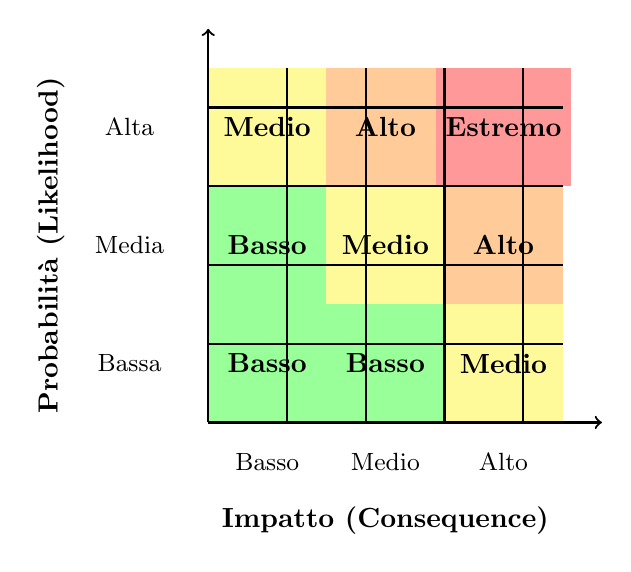
\begin{tikzpicture}[
    cell/.style={minimum size=1.5cm, align=center, font=\bfseries},
    font=\small
]

% Y-axis Likelihood
\node at (-1, 0.75) {Bassa};
\node at (-1, 2.25) {Media};
\node at (-1, 3.75) {Alta};
\node[rotate=90, font=\bfseries] at (-2, 2.25) {Probabilità (Likelihood)};

% X-axis Impact
\node at (0.75, -0.5) {Basso};
\node at (2.25, -0.5) {Medio};
\node at (3.75, -0.5) {Alto};
\node[font=\bfseries] at (2.25, -1.25) {Impatto (Consequence)};

% Row 1 (Bottom)
\node[cell, fill=green!40] at (0.75, 0.75) {Basso};
\node[cell, fill=green!40] at (2.25, 0.75) {Basso};
\node[cell, fill=yellow!40] at (3.75, 0.75) {Medio};

% Row 2 (Middle)
\node[cell, fill=green!40] at (0.75, 2.25) {Basso};
\node[cell, fill=yellow!40] at (2.25, 2.25) {Medio};
\node[cell, fill=orange!40] at (3.75, 2.25) {Alto};

% Row 3 (Top)
\node[cell, fill=yellow!40] at (0.75, 3.75) {Medio};
\node[cell, fill=orange!40] at (2.25, 3.75) {Alto};
\node[cell, fill=red!40] at (3.75, 3.75) {Estremo};

% Grid
\draw[thick] (0,0) grid (4.5, 4.5);
\draw[->, thick] (0,0) -- (0, 5);
\draw[->, thick] (0,0) -- (5, 0);

\end{tikzpicture}
\end{center}

Tutti i risultati confluiscono in un documento formale e costantemente aggiornato chiamato \textbf{Registro dei Rischi} (\textit{Risk Register}).

\begin{exbox}[Le Strategie di Trattamento del Rischio]
\begin{enumerate}
    \item \textbf{Riduzione della Probabilità (\textit{Mitigation}):} Implementazione di controlli preventivi (es. firewall, processi di \textit{patching} regolari, MFA) per rendere l'attacco o l'errore più difficile e improbabile.
    \item \textbf{Riduzione dell'Impatto:} Implementazione di controlli correttivi o di resilienza (es. backup archiviati \textit{offline}) che limitano il danno a evento avvenuto.
    \item \textbf{Trasferimento del Rischio (\textit{Transfer}):} Spostamento dell'onere finanziario o operativo su terzi (es. stipula di polizze assicurative \textit{cyber} o \textit{outsourcing} di servizi critici a provider Cloud qualificati con SLA stringenti).
    \item \textbf{Evitamento del Rischio (\textit{Avoidance}):} Dismissione completa del sistema, del processo di business o della tecnologia che genera il rischio, qualora i costi di mitigazione superino di gran lunga i benefici economici.
    \item \textbf{Accettazione del Rischio (\textit{Acceptance}):} Riconoscimento e approvazione formale del rischio residuo da parte del \textit{Senior Management} senza ulteriori azioni di mitigazione. Viene tipicamente applicato quando il rischio è già al di sotto dell'appetito aziendale o quando il costo dei controlli necessari eccede il valore reale dell'asset da proteggere.
\end{enumerate}
\end{exbox}
